\documentclass[beamer]{standalone}
\usepackage{../templates/common}
\usepackage{../templates/phylofig}

\begin{document}
\begin{standaloneframe}
\centering
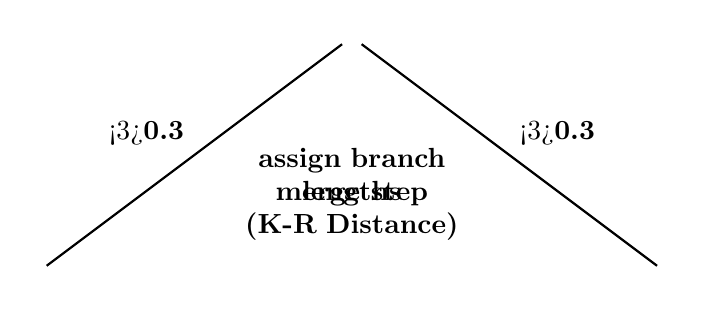
\begin{tikzpicture}
\phylofig{0,0}{ {0.3}{0.4}{0.1}{0.2}{0.0} }{}
\phylofig{8,0}{ {0.1}{0.5}{0.1}{0.2}{0.1} }{}

\onslide<2->{
\phylofig{4,5}{ {0.2}{0.45}{0.1}{0.2}{0.05} }{}
\phylofig{4,5-.2}{ { }{ }{ }{ }{ } }{}
\node (a) at (2,1) {};
\node (b) at (10,1) {};
\node (x) at (6,4) {};
\path (a) edge[thick] node[above left] {\only<3>{\textbf{0.3}}} (x);
\path (b) edge[thick] node[above right] {\only<3>{\textbf{0.3}}}(x);
}
\onslide<2>{\node(mrg) at (6,2) {\textbf{merge step}};}
\onslide<3>{\node at (6,2) [align=center,text width=3cm]{\textbf{assign branch lengths\\  (K-R Distance)}};}
\end{tikzpicture}
\end{standaloneframe}
\end{document}
